
% LaTeX file for generating the Model Description Table in Fig. 5 of
%
%  Nordlie E, Gewaltig M-O, Plesser HE (2009)
%  Towards Reproducible Descriptions of Neuronal Network Models.
%  PLoS Comput Biol 5(8): e1000456.
%
%  Paper URL : http://dx.doi.org/10.1371/journal.pcbi.1000456
%  Figure URL: http://dx.doi.org/10.1371/journal.pcbi.1000456.g005
%
% This file is released under a
%
%   Creative Commons Attribution, non-commercial, share-alike licence
%   http://creativecommons.org/licenses/by-nc-sa/3.0/de/deed.en
%
% with the following specifications:
%
%  1. When publishing tables generated from this LaTeX file and modified
%     versions of it, you must cite the paper by Nordlie et al given above.
%
%  2. The non-commercial clause applies only to the distribution of THIS FILE
%     and LaTeX source code files derived from it. You may commercially publish
%     documents generated using this file and derivatived versions of this file.
%
% Contact: Hans Ekkehard Plesser, UMB (hans.ekkehard.plesser at umb.no)

\documentclass{article}
% User defined commands
\input{../../../../thesis/manuscript/user-defined}

\input{../../../../thesis/manuscript/glossary}
\usepackage[margin=0.2in]{geometry} % get enough space on page

\usepackage{tabularx}  % automatically adjusts column width in tables
\usepackage{multirow}  % allows entries spanning several rows
\usepackage{colortbl}  % allows coloring tables
%\usepackage{natbib}
%\usepackage[fleqn]{amsmath}   % displayed equations flush left
%\setlength{\mathindent}{0em}

% use Helvetica for text, Pazo math fonts
\usepackage{mathpazo}
\usepackage[scaled=.95]{helvet}
\renewcommand\familydefault{\sfdefault}

\renewcommand\arraystretch{1.2}  % slightly more space in tables

\pagestyle{empty}  % no header of footer

% \hdr{ncols}{label}{title}
%
% Typeset header bar across table with ncols columns
% with label at left margin and centered title
%
\newcommand{\hdr}[3]{%
\multicolumn{#1}{|l|}{%
\color{white}\cellcolor[gray]{0.0}%
\textbf{\makebox[0pt]{#2}\hspace{0.5\linewidth}\makebox[0pt][c]{#3}}%
}%
}

%\graphicspath{{../../soma/netmod/cnstellate/DS_ClickRecovery/}{../../soma/netmod/cnstellate/}}

\begin{document}

prospective

\includegraphics[keepaspectratio=true,angle=-90,width=0.6\textwidth]{DS_ClickRecovery_result.0.eps}\clearpage
\includegraphics[keepaspectratio=true,angle=-90,width=0.6\textwidth]{DS_ClickRecovery_result.1.eps}\clearpage
\includegraphics[keepaspectratio=true,angle=-90,width=0.6\textwidth]{DS_ClickRecovery_result.2.eps}\clearpage
\includegraphics[keepaspectratio=true,angle=-90,width=0.6\textwidth]{DS_ClickRecovery_result.3.eps}\clearpage
\includegraphics[keepaspectratio=true,angle=-90,width=0.6\textwidth]{DS_ClickRecovery_result.4.eps}\clearpage
\includegraphics[keepaspectratio=true,angle=-90,width=0.6\textwidth]{DS_ClickRecovery_result.5.eps}\clearpage
\includegraphics[keepaspectratio=true,angle=-90,width=0.6\textwidth]{DS_ClickRecovery_result.6.eps}\clearpage
\includegraphics[keepaspectratio=true,angle=-90,width=0.6\textwidth]{DS_ClickRecovery_result.7.eps}\clearpage
\includegraphics[keepaspectratio=true,angle=-90,width=0.6\textwidth]{DS_ClickRecovery_result.8.eps}\clearpage
\includegraphics[keepaspectratio=true,angle=-90,width=0.6\textwidth]{DS_ClickRecovery_result.9.eps}\clearpage
\includegraphics[keepaspectratio=true,angle=-90,width=0.6\textwidth]{DS_ClickRecovery_result.10.eps}\clearpage
\includegraphics[keepaspectratio=true,angle=-90,width=0.6\textwidth]{DS_ClickRecovery_result.11.eps}\clearpage
\includegraphics[keepaspectratio=true,angle=-90,width=0.6\textwidth]{DS_ClickRecovery_result.12.eps}\clearpage
\includegraphics[keepaspectratio=true,angle=-90,width=0.6\textwidth]{DS_ClickRecovery_result.13.eps}\clearpage
\includegraphics[keepaspectratio=true,angle=-90,width=0.6\textwidth]{DS_ClickRecovery_result.14.eps}\clearpage
\includegraphics[keepaspectratio=true,angle=-90,width=0.6\textwidth]{DS_ClickRecovery_result.15.eps}\clearpage
\includegraphics[keepaspectratio=true,angle=-90,width=0.6\textwidth]{DS_ClickRecovery_result.16.eps}\clearpage
\includegraphics[keepaspectratio=true,angle=-90,width=0.6\textwidth]{DS_ClickRecovery_result.17.eps}\clearpage
\includegraphics[keepaspectratio=true,angle=-90,width=0.6\textwidth]{DS_ClickRecovery_result.18.eps}\clearpage
\includegraphics[keepaspectratio=true,angle=-90,width=0.6\textwidth]{DS_ClickRecovery_result.19.eps}\clearpage
\includegraphics[keepaspectratio=true,angle=-90,width=0.6\textwidth]{DS_ClickRecovery_result.20.eps}\clearpage



\includegraphics[keepaspectratio=true,angle=-90,width=0.6\textwidth]{DS_ClickRecovery_result.21.eps}\clearpage
\includegraphics[keepaspectratio=true,angle=-90,width=0.6\textwidth]{DS_ClickRecovery_result.22.eps}\clearpage
\includegraphics[keepaspectratio=true,angle=-90,width=0.6\textwidth]{DS_ClickRecovery_result.23.eps}\clearpage
\includegraphics[keepaspectratio=true,angle=-90,width=0.6\textwidth]{DS_ClickRecovery_result.24.eps}\clearpage
\includegraphics[keepaspectratio=true,angle=-90,width=0.6\textwidth]{DS_ClickRecovery_result.25.eps}\clearpage
\includegraphics[keepaspectratio=true,angle=-90,width=0.6\textwidth]{DS_ClickRecovery_result.26.eps}\clearpage
\includegraphics[keepaspectratio=true,angle=-90,width=0.6\textwidth]{DS_ClickRecovery_result.27.eps}\clearpage
\includegraphics[keepaspectratio=true,angle=-90,width=0.6\textwidth]{DS_ClickRecovery_result.28.eps}\clearpage
\includegraphics[keepaspectratio=true,angle=-90,width=0.6\textwidth]{DS_ClickRecovery_result.29.eps}\clearpage
\includegraphics[keepaspectratio=true,angle=-90,width=0.6\textwidth]{DS_ClickRecovery_result.30.eps}\clearpage
\includegraphics[keepaspectratio=true,angle=-90,width=0.6\textwidth]{DS_ClickRecovery_result.31.eps}\clearpage
\includegraphics[keepaspectratio=true,angle=-90,width=0.6\textwidth]{DS_ClickRecovery_result.32.eps}\clearpage
\includegraphics[keepaspectratio=true,angle=-90,width=0.6\textwidth]{DS_ClickRecovery_result.33.eps}\clearpage
\includegraphics[keepaspectratio=true,angle=-90,width=0.6\textwidth]{DS_ClickRecovery_result.34.eps}\clearpage
\includegraphics[keepaspectratio=true,angle=-90,width=0.6\textwidth]{DS_ClickRecovery_result.35.eps}\clearpage
\includegraphics[keepaspectratio=true,angle=-90,width=0.6\textwidth]{DS_ClickRecovery_result.36.eps}\clearpage
\includegraphics[keepaspectratio=true,angle=-90,width=0.6\textwidth]{DS_ClickRecovery_result.37.eps}\clearpage
\includegraphics[keepaspectratio=true,angle=-90,width=0.6\textwidth]{DS_ClickRecovery_result.38.eps}\clearpage
\includegraphics[keepaspectratio=true,angle=-90,width=0.6\textwidth]{DS_ClickRecovery_result.39.eps}\clearpage
\includegraphics[keepaspectratio=true,angle=-90,width=0.6\textwidth]{DS_ClickRecovery_result.40.eps}\clearpage




%%%%%%%%%%%%%%%%%%%%%%%%%%%%%%%%%%%%%%%%%%%%%%%%%%%%%%
% \bibliographystyle{plainnat}%bmc_article} % Style BST file
% \bibliography{../manuscript/bib/MyBib}

\end{document} 